\documentclass{standalone}
\usepackage{graphicx}	
\usepackage{amssymb, amsmath}
\usepackage{color}

\usepackage{tikz}
\usetikzlibrary{intersections, backgrounds, math}
\usepackage{pgfmath}

\definecolor{light}{RGB}{220, 188, 188}
\definecolor{mid}{RGB}{185, 124, 124}
\definecolor{dark}{RGB}{143, 39, 39}
\definecolor{highlight}{RGB}{180, 31, 180}
\definecolor{gray10}{gray}{0.1}
\definecolor{gray20}{gray}{0.2}
\definecolor{gray30}{gray}{0.3}
\definecolor{gray40}{gray}{0.4}
\definecolor{gray60}{gray}{0.6}
\definecolor{gray70}{gray}{0.7}
\definecolor{gray80}{gray}{0.8}
\definecolor{gray90}{gray}{0.9}
\definecolor{gray95}{gray}{0.95}


\begin{document}

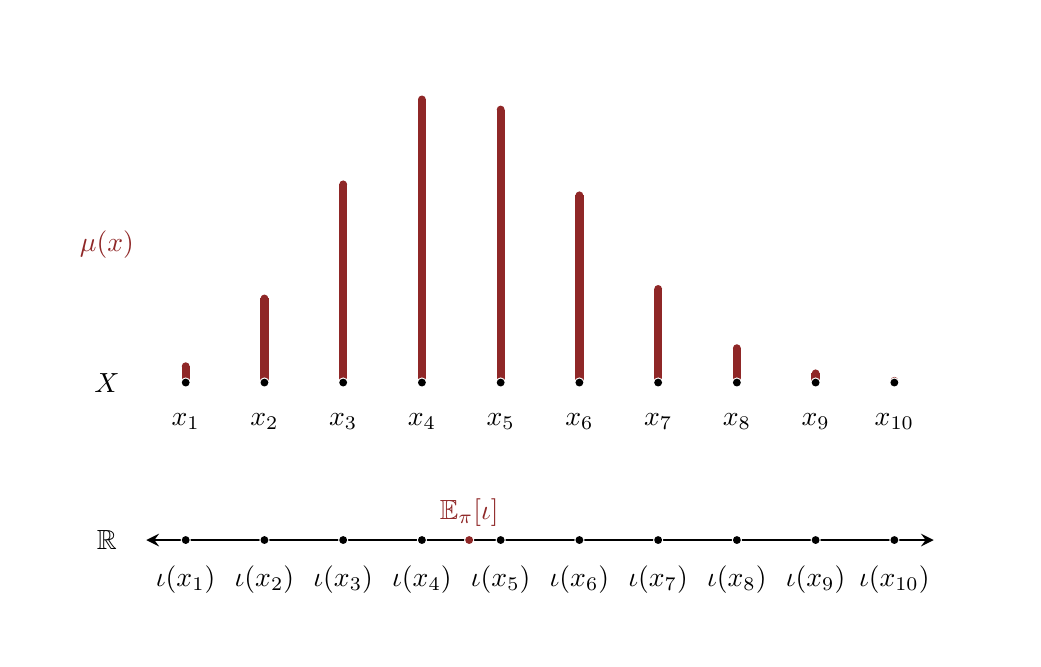
\begin{tikzpicture}[scale=1]
  \begin{scope}[shift={(0, 0)}]
    \draw[white] (-8, -5.25) rectangle (4.5, 2.5);
    
    \draw[<->, >=stealth, line width=1] (-6.5, -4) -- (3.5, -4);
    
    \foreach [count=\n] \m in {0.013841, 0.071184, 0.167790, 0.239700, 
                               0.231140, 0.158496, 0.079248, 0.029111, 
                               0.007798, 0.001485} {
      \pgfmathsetmacro{\x}{(\n - 1) - 6};
      \draw[dark, line width=3] (\x, -2) -- (\x, {(15 * \m - 2)});
      \fill[dark] (\x, {(15 * \m - 2)}) circle (0.05);
      \fill[white] (\x, -2) circle (0.065);
      \fill[black] (\x, -2) circle (0.05);
      \node at (\x, -2.5) { $x_{\n}$ };
      
      \fill[white] (\x, -4) circle (0.065);
      \fill[black] (\x, -4) circle (0.05);
      \node at (\x, -4.5) { $\iota(x_{\n})$ };
    }
 
    \node[dark] at (-6 + 3.6, -3.65) { $\mathbb{E}_{\pi}[\iota]$ };
    \fill[white] (-6 + 3.6, -4) circle (0.065);
    \fill[dark] (-6 + 3.6, -4) circle (0.05);
 
    \node[dark] at (-7, -0.25) { $\mu(x)$ };
    \node at (-7, -2) { $X$ };
    \node at (-7, -4) { $\mathbb{R}$ };
 
  \end{scope}
  
\end{tikzpicture}

\end{document}  